\documentclass[twoside]{book}

% Packages required by doxygen
\usepackage{fixltx2e}
\usepackage{calc}
\usepackage{doxygen}
\usepackage[export]{adjustbox} % also loads graphicx
\usepackage{graphicx}
\usepackage[utf8]{inputenc}
\usepackage{makeidx}
\usepackage{multicol}
\usepackage{multirow}
\PassOptionsToPackage{warn}{textcomp}
\usepackage{textcomp}
\usepackage[nointegrals]{wasysym}
\usepackage[table]{xcolor}

% NLS support packages
\usepackage[spanish]{babel}
% Font selection
\usepackage[T1]{fontenc}
\usepackage[scaled=.90]{helvet}
\usepackage{courier}
\usepackage{amssymb}
\usepackage{sectsty}
\renewcommand{\familydefault}{\sfdefault}
\allsectionsfont{%
  \fontseries{bc}\selectfont%
  \color{darkgray}%
}
\renewcommand{\DoxyLabelFont}{%
  \fontseries{bc}\selectfont%
  \color{darkgray}%
}
\newcommand{\+}{\discretionary{\mbox{\scriptsize$\hookleftarrow$}}{}{}}

% Page & text layout
\usepackage{geometry}
\geometry{%
  a4paper,%
  top=2.5cm,%
  bottom=2.5cm,%
  left=2.5cm,%
  right=2.5cm%
}
\tolerance=750
\hfuzz=15pt
\hbadness=750
\setlength{\emergencystretch}{15pt}
\setlength{\parindent}{0cm}
\setlength{\parskip}{3ex plus 2ex minus 2ex}
\makeatletter
\renewcommand{\paragraph}{%
  \@startsection{paragraph}{4}{0ex}{-1.0ex}{1.0ex}{%
    \normalfont\normalsize\bfseries\SS@parafont%
  }%
}
\renewcommand{\subparagraph}{%
  \@startsection{subparagraph}{5}{0ex}{-1.0ex}{1.0ex}{%
    \normalfont\normalsize\bfseries\SS@subparafont%
  }%
}
\makeatother

% Headers & footers
\usepackage{fancyhdr}
\pagestyle{fancyplain}
\fancyhead[LE]{\fancyplain{}{\bfseries\thepage}}
\fancyhead[CE]{\fancyplain{}{}}
\fancyhead[RE]{\fancyplain{}{\bfseries\leftmark}}
\fancyhead[LO]{\fancyplain{}{\bfseries\rightmark}}
\fancyhead[CO]{\fancyplain{}{}}
\fancyhead[RO]{\fancyplain{}{\bfseries\thepage}}
\fancyfoot[LE]{\fancyplain{}{}}
\fancyfoot[CE]{\fancyplain{}{}}
\fancyfoot[RE]{\fancyplain{}{\bfseries\scriptsize Generado por Doxygen }}
\fancyfoot[LO]{\fancyplain{}{\bfseries\scriptsize Generado por Doxygen }}
\fancyfoot[CO]{\fancyplain{}{}}
\fancyfoot[RO]{\fancyplain{}{}}
\renewcommand{\footrulewidth}{0.4pt}
\renewcommand{\chaptermark}[1]{%
  \markboth{#1}{}%
}
\renewcommand{\sectionmark}[1]{%
  \markright{\thesection\ #1}%
}

% Indices & bibliography
\usepackage{natbib}
\usepackage[titles]{tocloft}
\setcounter{tocdepth}{3}
\setcounter{secnumdepth}{5}
\makeindex

% Hyperlinks (required, but should be loaded last)
\usepackage{ifpdf}
\ifpdf
  \usepackage[pdftex,pagebackref=true]{hyperref}
\else
  \usepackage[ps2pdf,pagebackref=true]{hyperref}
\fi
\hypersetup{%
  colorlinks=true,%
  linkcolor=blue,%
  citecolor=blue,%
  unicode%
}

% Custom commands
\newcommand{\clearemptydoublepage}{%
  \newpage{\pagestyle{empty}\cleardoublepage}%
}

\usepackage{caption}
\captionsetup{labelsep=space,justification=centering,font={bf},singlelinecheck=off,skip=4pt,position=top}

%===== C O N T E N T S =====

\begin{document}

% Titlepage & ToC
\hypersetup{pageanchor=false,
             bookmarksnumbered=true,
             pdfencoding=unicode
            }
\pagenumbering{alph}
\begin{titlepage}
\vspace*{7cm}
\begin{center}%
{\Large Aplicación para codificar y decodificar textos escritos en diversos idiomas (Práctica P\+R\+O2) \\[1ex]\large 24/4/2019 }\\
\vspace*{1cm}
{\large Generado por Doxygen 1.8.13}\\
\end{center}
\end{titlepage}
\clearemptydoublepage
\pagenumbering{roman}
\tableofcontents
\clearemptydoublepage
\pagenumbering{arabic}
\hypersetup{pageanchor=true}

%--- Begin generated contents ---
\chapter{Página principal}
\label{index}\hypertarget{index}{}Este documento html documenta la especificación de un codificador/decodificador de mensajes. El programa principal se encuentra en el archivo main.\+cc. A parte de este archivo también són necesarias la siguientes 4 clases\+:~\newline
 -\/{\bfseries \hyperlink{cjt__idioma_8hh}{cjt\+\_\+idioma.\+hh}} que se encarga de gestionar conjuntos de idiomas~\newline
 -\/{\bfseries \hyperlink{idioma_8hh}{idioma.\+hh}} con el que podemos definir un nuevo idioma a partir de un nombre y una tabla de frecuencias.~\newline
 -\/{\bfseries \hyperlink{treecode_8hh}{treecode.\+hh}} que se encarga de traducir las tablas de frecuencias a arbol binario y después codificar/decodificar mensajes recorriendo los árboles.~\newline
 -\/{\bfseries \hyperlink{tabla_8hh}{tabla.\+hh}} se encarga de leer,almacenar y escribir las tablas de frecuencias.~\newline
 
\chapter{Índice de clases}
\section{Lista de clases}
Lista de las clases, estructuras, uniones e interfaces con una breve descripción\+:\begin{DoxyCompactList}
\item\contentsline{section}{\hyperlink{classcjt__idioma}{cjt\+\_\+idioma} \\*Representa un conjunto de idomas }{\pageref{classcjt__idioma}}{}
\item\contentsline{section}{\hyperlink{classidioma}{idioma} \\*Representa un idoma }{\pageref{classidioma}}{}
\item\contentsline{section}{\hyperlink{classtabla}{tabla} \\*Representa la tabla de frecuencias de un idioma }{\pageref{classtabla}}{}
\item\contentsline{section}{\hyperlink{classtreecode}{treecode} \\*Representa el treecode de un idioma }{\pageref{classtreecode}}{}
\end{DoxyCompactList}

\chapter{Indice de archivos}
\section{Lista de archivos}
Lista de todos los archivos con descripciones breves\+:\begin{DoxyCompactList}
\item\contentsline{section}{\hyperlink{cjt__idioma_8hh}{cjt\+\_\+idioma.\+hh} \\*Especificación de la clase cjt\+\_\+dioma }{\pageref{cjt__idioma_8hh}}{}
\item\contentsline{section}{\hyperlink{idioma_8hh}{idioma.\+hh} \\*Especificación de la clase idioma }{\pageref{idioma_8hh}}{}
\item\contentsline{section}{\hyperlink{program_8cc}{program.\+cc} \\*Programa principal }{\pageref{program_8cc}}{}
\item\contentsline{section}{\hyperlink{tabla_8hh}{tabla.\+hh} \\*Especificación de la clase tabla }{\pageref{tabla_8hh}}{}
\item\contentsline{section}{\hyperlink{treecode_8hh}{treecode.\+hh} \\*Especificación de la clase treecode }{\pageref{treecode_8hh}}{}
\end{DoxyCompactList}

\chapter{Documentación de las clases}
\hypertarget{classcjt__idioma}{}\section{Referencia de la Clase cjt\+\_\+idioma}
\label{classcjt__idioma}\index{cjt\+\_\+idioma@{cjt\+\_\+idioma}}


Representa un conjunto de idomas.  


\subsection*{Métodos públicos}
\begin{DoxyCompactItemize}
\item 
\hyperlink{classcjt__idioma_a79c18a172e61c3276f352a81c479dfb8}{cjt\+\_\+idioma} ()
\begin{DoxyCompactList}\small\item\em Crea un conjunto de idiomas. \end{DoxyCompactList}\item 
bool \hyperlink{classcjt__idioma_a253fbf0732efc679dea434ee7d261ffa}{existe\+\_\+idioma} (const string \&i)
\begin{DoxyCompactList}\small\item\em Consulta si existe un idioma en el conjunto con el nombre del parámetro. \end{DoxyCompactList}\item 
void \hyperlink{classcjt__idioma_aaf8acea2625eb1a72fbeaed23357c4ad}{anadir\+\_\+idioma} (const string \&s)
\begin{DoxyCompactList}\small\item\em Se añade al conjunto un nuevo idioma. \end{DoxyCompactList}\item 
void \hyperlink{classcjt__idioma_ac9cdce411a32c42a9fc7da848f7de4c0}{modificar\+\_\+idioma} (const string \&i)
\begin{DoxyCompactList}\small\item\em Modifica un idioma. \end{DoxyCompactList}\item 
void \hyperlink{classcjt__idioma_a5a92374dcbb5b9a0af7fdfccb59bc423}{codifica} (const string \&nombre, string \&texto)
\begin{DoxyCompactList}\small\item\em Codifica un mensaje en un idioma. \end{DoxyCompactList}\item 
void \hyperlink{classcjt__idioma_a25ee22b5af84a8ce22de2cee8128a08c}{decodifica} (const string \&nombre, const string \&texto)
\begin{DoxyCompactList}\small\item\em Decodifica un mensaje en un idioma. \end{DoxyCompactList}\item 
void \hyperlink{classcjt__idioma_ae2ab9ad48166bad14e113f748d1a888c}{consultar\+\_\+tabla\+\_\+de\+\_\+frequencias} (const string \&i)
\begin{DoxyCompactList}\small\item\em Consulta la tabla de frecuencias de un idioma. \end{DoxyCompactList}\item 
void \hyperlink{classcjt__idioma_a2d13a4e69a358756359ee6e262de2fb0}{consultar\+\_\+treecode} (const string \&i)
\begin{DoxyCompactList}\small\item\em Consulta el treecodede un idioma. \end{DoxyCompactList}\item 
void \hyperlink{classcjt__idioma_a2e4b954ce7ee66596412c335430e9be8}{consultar\+\_\+codigos} (const string \&s)
\begin{DoxyCompactList}\small\item\em Consulta uno o todos los codigios de un idioma. \end{DoxyCompactList}\end{DoxyCompactItemize}


\subsection{Descripción detallada}
Representa un conjunto de idomas. 

Contiene los idiomas y operaciones de gestión del conjunto. 

Definición en la línea 22 del archivo cjt\+\_\+idioma.\+hh.



\subsection{Documentación del constructor y destructor}
\mbox{\Hypertarget{classcjt__idioma_a79c18a172e61c3276f352a81c479dfb8}\label{classcjt__idioma_a79c18a172e61c3276f352a81c479dfb8}} 
\index{cjt\+\_\+idioma@{cjt\+\_\+idioma}!cjt\+\_\+idioma@{cjt\+\_\+idioma}}
\index{cjt\+\_\+idioma@{cjt\+\_\+idioma}!cjt\+\_\+idioma@{cjt\+\_\+idioma}}
\subsubsection{\texorpdfstring{cjt\+\_\+idioma()}{cjt\_idioma()}}
{\footnotesize\ttfamily cjt\+\_\+idioma\+::cjt\+\_\+idioma (\begin{DoxyParamCaption}{ }\end{DoxyParamCaption})}



Crea un conjunto de idiomas. 

\begin{DoxyPrecond}{Precondición}
Cierto 
\end{DoxyPrecond}
\begin{DoxyPostcond}{Postcondición}
Se ha creado un conjunto de idiomas vacio. 
\end{DoxyPostcond}


\subsection{Documentación de las funciones miembro}
\mbox{\Hypertarget{classcjt__idioma_a253fbf0732efc679dea434ee7d261ffa}\label{classcjt__idioma_a253fbf0732efc679dea434ee7d261ffa}} 
\index{cjt\+\_\+idioma@{cjt\+\_\+idioma}!existe\+\_\+idioma@{existe\+\_\+idioma}}
\index{existe\+\_\+idioma@{existe\+\_\+idioma}!cjt\+\_\+idioma@{cjt\+\_\+idioma}}
\subsubsection{\texorpdfstring{existe\+\_\+idioma()}{existe\_idioma()}}
{\footnotesize\ttfamily bool cjt\+\_\+idioma\+::existe\+\_\+idioma (\begin{DoxyParamCaption}\item[{const string \&}]{i }\end{DoxyParamCaption})}



Consulta si existe un idioma en el conjunto con el nombre del parámetro. 

\begin{DoxyPrecond}{Precondición}
i contiene el nombre del idioma a consultar. 
\end{DoxyPrecond}
\begin{DoxyPostcond}{Postcondición}
Se retorna cierto si el idoma existe, falso en caso contario. 
\end{DoxyPostcond}
\mbox{\Hypertarget{classcjt__idioma_aaf8acea2625eb1a72fbeaed23357c4ad}\label{classcjt__idioma_aaf8acea2625eb1a72fbeaed23357c4ad}} 
\index{cjt\+\_\+idioma@{cjt\+\_\+idioma}!anadir\+\_\+idioma@{anadir\+\_\+idioma}}
\index{anadir\+\_\+idioma@{anadir\+\_\+idioma}!cjt\+\_\+idioma@{cjt\+\_\+idioma}}
\subsubsection{\texorpdfstring{anadir\+\_\+idioma()}{anadir\_idioma()}}
{\footnotesize\ttfamily void cjt\+\_\+idioma\+::anadir\+\_\+idioma (\begin{DoxyParamCaption}\item[{const string \&}]{s }\end{DoxyParamCaption})}



Se añade al conjunto un nuevo idioma. 

\begin{DoxyPrecond}{Precondición}
s contiene el nombre del idioma a añadir. 
\end{DoxyPrecond}
\begin{DoxyPostcond}{Postcondición}
se ha añadido el idioma de nombre s al conjunto c. 
\end{DoxyPostcond}
\mbox{\Hypertarget{classcjt__idioma_ac9cdce411a32c42a9fc7da848f7de4c0}\label{classcjt__idioma_ac9cdce411a32c42a9fc7da848f7de4c0}} 
\index{cjt\+\_\+idioma@{cjt\+\_\+idioma}!modificar\+\_\+idioma@{modificar\+\_\+idioma}}
\index{modificar\+\_\+idioma@{modificar\+\_\+idioma}!cjt\+\_\+idioma@{cjt\+\_\+idioma}}
\subsubsection{\texorpdfstring{modificar\+\_\+idioma()}{modificar\_idioma()}}
{\footnotesize\ttfamily void cjt\+\_\+idioma\+::modificar\+\_\+idioma (\begin{DoxyParamCaption}\item[{const string \&}]{i }\end{DoxyParamCaption})}



Modifica un idioma. 

\begin{DoxyPrecond}{Precondición}
i contiene el nombre del idioma a modificar, i existe en c. 
\end{DoxyPrecond}
\begin{DoxyPostcond}{Postcondición}
se ha modificado el idioma. 
\end{DoxyPostcond}
\mbox{\Hypertarget{classcjt__idioma_a5a92374dcbb5b9a0af7fdfccb59bc423}\label{classcjt__idioma_a5a92374dcbb5b9a0af7fdfccb59bc423}} 
\index{cjt\+\_\+idioma@{cjt\+\_\+idioma}!codifica@{codifica}}
\index{codifica@{codifica}!cjt\+\_\+idioma@{cjt\+\_\+idioma}}
\subsubsection{\texorpdfstring{codifica()}{codifica()}}
{\footnotesize\ttfamily void cjt\+\_\+idioma\+::codifica (\begin{DoxyParamCaption}\item[{const string \&}]{nombre,  }\item[{string \&}]{texto }\end{DoxyParamCaption})}



Codifica un mensaje en un idioma. 

\begin{DoxyPrecond}{Precondición}
nombre contiene el idioma en el que codificar y texto el mensaje a codificar. 
\end{DoxyPrecond}
\begin{DoxyPostcond}{Postcondición}
Si se puede codificar, se ha escrito por el canal estandard de salida el mensaje codificado. En caso contrario el usuario es informado de la situación. 
\end{DoxyPostcond}
\mbox{\Hypertarget{classcjt__idioma_a25ee22b5af84a8ce22de2cee8128a08c}\label{classcjt__idioma_a25ee22b5af84a8ce22de2cee8128a08c}} 
\index{cjt\+\_\+idioma@{cjt\+\_\+idioma}!decodifica@{decodifica}}
\index{decodifica@{decodifica}!cjt\+\_\+idioma@{cjt\+\_\+idioma}}
\subsubsection{\texorpdfstring{decodifica()}{decodifica()}}
{\footnotesize\ttfamily void cjt\+\_\+idioma\+::decodifica (\begin{DoxyParamCaption}\item[{const string \&}]{nombre,  }\item[{const string \&}]{texto }\end{DoxyParamCaption})}



Decodifica un mensaje en un idioma. 

\begin{DoxyPrecond}{Precondición}
nombre contiene el idioma en el que decodificar y texto el mensaje a decodificar. 
\end{DoxyPrecond}
\begin{DoxyPostcond}{Postcondición}
Si se puede decodificar, se ha escrito por el canal estandard de salida el mensaje decodificado. En caso contrario el usuario es informado de la situación. 
\end{DoxyPostcond}
\mbox{\Hypertarget{classcjt__idioma_ae2ab9ad48166bad14e113f748d1a888c}\label{classcjt__idioma_ae2ab9ad48166bad14e113f748d1a888c}} 
\index{cjt\+\_\+idioma@{cjt\+\_\+idioma}!consultar\+\_\+tabla\+\_\+de\+\_\+frequencias@{consultar\+\_\+tabla\+\_\+de\+\_\+frequencias}}
\index{consultar\+\_\+tabla\+\_\+de\+\_\+frequencias@{consultar\+\_\+tabla\+\_\+de\+\_\+frequencias}!cjt\+\_\+idioma@{cjt\+\_\+idioma}}
\subsubsection{\texorpdfstring{consultar\+\_\+tabla\+\_\+de\+\_\+frequencias()}{consultar\_tabla\_de\_frequencias()}}
{\footnotesize\ttfamily void cjt\+\_\+idioma\+::consultar\+\_\+tabla\+\_\+de\+\_\+frequencias (\begin{DoxyParamCaption}\item[{const string \&}]{i }\end{DoxyParamCaption})}



Consulta la tabla de frecuencias de un idioma. 

\begin{DoxyPrecond}{Precondición}
i contiene el nombre del idioma del que queremos ver la tabla de frecuencias, i existe en c. 
\end{DoxyPrecond}
\begin{DoxyPostcond}{Postcondición}
se ha escrito por el canal estandard de salida la tabla de frecuencias. 
\end{DoxyPostcond}
\mbox{\Hypertarget{classcjt__idioma_a2d13a4e69a358756359ee6e262de2fb0}\label{classcjt__idioma_a2d13a4e69a358756359ee6e262de2fb0}} 
\index{cjt\+\_\+idioma@{cjt\+\_\+idioma}!consultar\+\_\+treecode@{consultar\+\_\+treecode}}
\index{consultar\+\_\+treecode@{consultar\+\_\+treecode}!cjt\+\_\+idioma@{cjt\+\_\+idioma}}
\subsubsection{\texorpdfstring{consultar\+\_\+treecode()}{consultar\_treecode()}}
{\footnotesize\ttfamily void cjt\+\_\+idioma\+::consultar\+\_\+treecode (\begin{DoxyParamCaption}\item[{const string \&}]{i }\end{DoxyParamCaption})}



Consulta el treecodede un idioma. 

\begin{DoxyPrecond}{Precondición}
i contiene el nombre del idioma del que queremos ver el treecode, i existe en c. 
\end{DoxyPrecond}
\begin{DoxyPostcond}{Postcondición}
se ha escrito por el canal estandard de salida el treecode en prorden e inorden. 
\end{DoxyPostcond}
\mbox{\Hypertarget{classcjt__idioma_a2e4b954ce7ee66596412c335430e9be8}\label{classcjt__idioma_a2e4b954ce7ee66596412c335430e9be8}} 
\index{cjt\+\_\+idioma@{cjt\+\_\+idioma}!consultar\+\_\+codigos@{consultar\+\_\+codigos}}
\index{consultar\+\_\+codigos@{consultar\+\_\+codigos}!cjt\+\_\+idioma@{cjt\+\_\+idioma}}
\subsubsection{\texorpdfstring{consultar\+\_\+codigos()}{consultar\_codigos()}}
{\footnotesize\ttfamily void cjt\+\_\+idioma\+::consultar\+\_\+codigos (\begin{DoxyParamCaption}\item[{const string \&}]{s }\end{DoxyParamCaption})}



Consulta uno o todos los codigios de un idioma. 

\begin{DoxyPrecond}{Precondición}
s contiene el nombre del idioma del que queremos ver los codigos. En el canal estandard de entrada espera el caracter a consultaro la string \char`\"{}todos\char`\"{}. 
\end{DoxyPrecond}
\begin{DoxyPostcond}{Postcondición}
se ha escrito por el canal estandard de salida el codigo o codigos correspondientes. 
\end{DoxyPostcond}


La documentación para esta clase fue generada a partir del siguiente fichero\+:\begin{DoxyCompactItemize}
\item 
\hyperlink{cjt__idioma_8hh}{cjt\+\_\+idioma.\+hh}\end{DoxyCompactItemize}

\hypertarget{classidioma}{}\section{Referencia de la Clase idioma}
\label{classidioma}\index{idioma@{idioma}}


Representa un idoma.  


\subsection*{Métodos públicos}
\begin{DoxyCompactItemize}
\item 
\hyperlink{classidioma_aef8714e17b1c5141104f5fb7bd989283}{idioma} ()
\begin{DoxyCompactList}\small\item\em Crea un nuevo idioma. \end{DoxyCompactList}\item 
void \hyperlink{classidioma_a40b865628fe20757e63c10cecd516c1f}{crear\+\_\+idioma} ()
\begin{DoxyCompactList}\small\item\em Crea un nuevo idioma. \end{DoxyCompactList}\item 
void \hyperlink{classidioma_af7d4b2d6a05e6b87783d9394fb1cc08e}{modificar\+\_\+idioma} ()
\begin{DoxyCompactList}\small\item\em Modifica un idioma. \end{DoxyCompactList}\item 
void \hyperlink{classidioma_ab1f4f36cf5bef660d93208ca12a08d15}{codifica} (string \&text)
\begin{DoxyCompactList}\small\item\em Codifica un texto. \end{DoxyCompactList}\item 
void \hyperlink{classidioma_a901e5b496773705624ae82bdcf15fac8}{decodifica} (const string \&texto)
\begin{DoxyCompactList}\small\item\em Decodifica un mensaje en un idioma. \end{DoxyCompactList}\item 
void \hyperlink{classidioma_a3b803dbdff20ebe884dd8e66550a856f}{consultar\+\_\+tabla} ()
\begin{DoxyCompactList}\small\item\em Consultar la tabla de frecuencias de un idioma. \end{DoxyCompactList}\item 
void \hyperlink{classidioma_aba4621fa2985a6ceba574eeeca069b8d}{consultar\+\_\+treecode} ()
\begin{DoxyCompactList}\small\item\em Consultar el treecode de un idioma. \end{DoxyCompactList}\item 
void \hyperlink{classidioma_a4e58f4dbc3845d4d8cea0c6b923a2e4e}{consultar\+\_\+codigos} ()
\begin{DoxyCompactList}\small\item\em Consultar los codigos de un idioma. \end{DoxyCompactList}\item 
void \hyperlink{classidioma_ad7342a94567fbd464ef2ee40ad1bb213}{consultar\+\_\+caracter} (const string \&car)
\begin{DoxyCompactList}\small\item\em Consulta el codigo de un caracter. \end{DoxyCompactList}\end{DoxyCompactItemize}


\subsection{Descripción detallada}
Representa un idoma. 

Contiene el nombre, la tabla de frecuencias y las operaciones sobre este como modificadoras o consultoras. 

Definición en la línea 19 del archivo idioma.\+hh.



\subsection{Documentación del constructor y destructor}
\mbox{\Hypertarget{classidioma_aef8714e17b1c5141104f5fb7bd989283}\label{classidioma_aef8714e17b1c5141104f5fb7bd989283}} 
\index{idioma@{idioma}!idioma@{idioma}}
\index{idioma@{idioma}!idioma@{idioma}}
\subsubsection{\texorpdfstring{idioma()}{idioma()}}
{\footnotesize\ttfamily idioma\+::idioma (\begin{DoxyParamCaption}{ }\end{DoxyParamCaption})}



Crea un nuevo idioma. 

\begin{DoxyPrecond}{Precondición}
cierto 
\end{DoxyPrecond}
\begin{DoxyPostcond}{Postcondición}
El resultado es un objeto de la clase idoma vacio. 
\end{DoxyPostcond}


\subsection{Documentación de las funciones miembro}
\mbox{\Hypertarget{classidioma_a40b865628fe20757e63c10cecd516c1f}\label{classidioma_a40b865628fe20757e63c10cecd516c1f}} 
\index{idioma@{idioma}!crear\+\_\+idioma@{crear\+\_\+idioma}}
\index{crear\+\_\+idioma@{crear\+\_\+idioma}!idioma@{idioma}}
\subsubsection{\texorpdfstring{crear\+\_\+idioma()}{crear\_idioma()}}
{\footnotesize\ttfamily void idioma\+::crear\+\_\+idioma (\begin{DoxyParamCaption}{ }\end{DoxyParamCaption})}



Crea un nuevo idioma. 

\begin{DoxyPrecond}{Precondición}
cierto 
\end{DoxyPrecond}
\begin{DoxyPostcond}{Postcondición}
Se ha creado un objeto de la clase idoma. 
\end{DoxyPostcond}
\mbox{\Hypertarget{classidioma_af7d4b2d6a05e6b87783d9394fb1cc08e}\label{classidioma_af7d4b2d6a05e6b87783d9394fb1cc08e}} 
\index{idioma@{idioma}!modificar\+\_\+idioma@{modificar\+\_\+idioma}}
\index{modificar\+\_\+idioma@{modificar\+\_\+idioma}!idioma@{idioma}}
\subsubsection{\texorpdfstring{modificar\+\_\+idioma()}{modificar\_idioma()}}
{\footnotesize\ttfamily void idioma\+::modificar\+\_\+idioma (\begin{DoxyParamCaption}{ }\end{DoxyParamCaption})}



Modifica un idioma. 

\begin{DoxyPrecond}{Precondición}
Cierto. 
\end{DoxyPrecond}
\begin{DoxyPostcond}{Postcondición}
Se ha modificado el idioma. 
\end{DoxyPostcond}
\mbox{\Hypertarget{classidioma_ab1f4f36cf5bef660d93208ca12a08d15}\label{classidioma_ab1f4f36cf5bef660d93208ca12a08d15}} 
\index{idioma@{idioma}!codifica@{codifica}}
\index{codifica@{codifica}!idioma@{idioma}}
\subsubsection{\texorpdfstring{codifica()}{codifica()}}
{\footnotesize\ttfamily void idioma\+::codifica (\begin{DoxyParamCaption}\item[{string \&}]{text }\end{DoxyParamCaption})}



Codifica un texto. 

\begin{DoxyPrecond}{Precondición}
en la string texto se encuentra el mensaje a codificar. 
\end{DoxyPrecond}
\begin{DoxyPostcond}{Postcondición}
Se ha escrito por el canal estandard de salida el mensaje codificado. 
\end{DoxyPostcond}
\mbox{\Hypertarget{classidioma_a901e5b496773705624ae82bdcf15fac8}\label{classidioma_a901e5b496773705624ae82bdcf15fac8}} 
\index{idioma@{idioma}!decodifica@{decodifica}}
\index{decodifica@{decodifica}!idioma@{idioma}}
\subsubsection{\texorpdfstring{decodifica()}{decodifica()}}
{\footnotesize\ttfamily void idioma\+::decodifica (\begin{DoxyParamCaption}\item[{const string \&}]{texto }\end{DoxyParamCaption})}



Decodifica un mensaje en un idioma. 

\begin{DoxyPrecond}{Precondición}
texto contiene el mensaje a decodificar. 
\end{DoxyPrecond}
\begin{DoxyPostcond}{Postcondición}
Si se puede decodificar, se ha escrito por el canal estandard de salida el mensaje decodificado. En caso contrario el usuario es informado de la situación. 
\end{DoxyPostcond}
\mbox{\Hypertarget{classidioma_a3b803dbdff20ebe884dd8e66550a856f}\label{classidioma_a3b803dbdff20ebe884dd8e66550a856f}} 
\index{idioma@{idioma}!consultar\+\_\+tabla@{consultar\+\_\+tabla}}
\index{consultar\+\_\+tabla@{consultar\+\_\+tabla}!idioma@{idioma}}
\subsubsection{\texorpdfstring{consultar\+\_\+tabla()}{consultar\_tabla()}}
{\footnotesize\ttfamily void idioma\+::consultar\+\_\+tabla (\begin{DoxyParamCaption}{ }\end{DoxyParamCaption})}



Consultar la tabla de frecuencias de un idioma. 

\begin{DoxyPrecond}{Precondición}
Cierto. 
\end{DoxyPrecond}
\begin{DoxyPostcond}{Postcondición}
Se ha escrito la tabla de frecuencias del parametro implícito. 
\end{DoxyPostcond}
\mbox{\Hypertarget{classidioma_aba4621fa2985a6ceba574eeeca069b8d}\label{classidioma_aba4621fa2985a6ceba574eeeca069b8d}} 
\index{idioma@{idioma}!consultar\+\_\+treecode@{consultar\+\_\+treecode}}
\index{consultar\+\_\+treecode@{consultar\+\_\+treecode}!idioma@{idioma}}
\subsubsection{\texorpdfstring{consultar\+\_\+treecode()}{consultar\_treecode()}}
{\footnotesize\ttfamily void idioma\+::consultar\+\_\+treecode (\begin{DoxyParamCaption}{ }\end{DoxyParamCaption})}



Consultar el treecode de un idioma. 

\begin{DoxyPrecond}{Precondición}
Cierto. 
\end{DoxyPrecond}
\begin{DoxyPostcond}{Postcondición}
Se ha escrito el treecode del parametro implícito. 
\end{DoxyPostcond}
\mbox{\Hypertarget{classidioma_a4e58f4dbc3845d4d8cea0c6b923a2e4e}\label{classidioma_a4e58f4dbc3845d4d8cea0c6b923a2e4e}} 
\index{idioma@{idioma}!consultar\+\_\+codigos@{consultar\+\_\+codigos}}
\index{consultar\+\_\+codigos@{consultar\+\_\+codigos}!idioma@{idioma}}
\subsubsection{\texorpdfstring{consultar\+\_\+codigos()}{consultar\_codigos()}}
{\footnotesize\ttfamily void idioma\+::consultar\+\_\+codigos (\begin{DoxyParamCaption}{ }\end{DoxyParamCaption})}



Consultar los codigos de un idioma. 

\begin{DoxyPrecond}{Precondición}
Cierto. 
\end{DoxyPrecond}
\begin{DoxyPostcond}{Postcondición}
Se ha escrito la tabla de codigos del parametro implícito. 
\end{DoxyPostcond}
\mbox{\Hypertarget{classidioma_ad7342a94567fbd464ef2ee40ad1bb213}\label{classidioma_ad7342a94567fbd464ef2ee40ad1bb213}} 
\index{idioma@{idioma}!consultar\+\_\+caracter@{consultar\+\_\+caracter}}
\index{consultar\+\_\+caracter@{consultar\+\_\+caracter}!idioma@{idioma}}
\subsubsection{\texorpdfstring{consultar\+\_\+caracter()}{consultar\_caracter()}}
{\footnotesize\ttfamily void idioma\+::consultar\+\_\+caracter (\begin{DoxyParamCaption}\item[{const string \&}]{car }\end{DoxyParamCaption})}



Consulta el codigo de un caracter. 

\begin{DoxyPrecond}{Precondición}
car contiene el caracter a consultar. 
\end{DoxyPrecond}
\begin{DoxyPostcond}{Postcondición}
Se ha escrito el codigo de car. 
\end{DoxyPostcond}


La documentación para esta clase fue generada a partir del siguiente fichero\+:\begin{DoxyCompactItemize}
\item 
\hyperlink{idioma_8hh}{idioma.\+hh}\end{DoxyCompactItemize}

\hypertarget{classtabla}{}\section{Referencia de la Clase tabla}
\label{classtabla}\index{tabla@{tabla}}


Representa la tabla de frecuencias de un idioma.  


\subsection*{Métodos públicos}
\begin{DoxyCompactItemize}
\item 
\hyperlink{classtabla_a47ec7f5106829c96469acb80c4992849}{tabla} ()
\item 
void \hyperlink{classtabla_ab297ddbd500d85a98d7c801697b73721}{leer} ()
\begin{DoxyCompactList}\small\item\em Lee una tabla. \end{DoxyCompactList}\item 
void \hyperlink{classtabla_a37f915651b80eaa0c6dc47c23ff92557}{modificar} ()
\begin{DoxyCompactList}\small\item\em Escribe una tabla. \end{DoxyCompactList}\item 
void \hyperlink{classtabla_ae0d9d7c8c80ef904a0c6cb0d25268b21}{escribir} ()
\begin{DoxyCompactList}\small\item\em Consulta la tabla de frecuencias de un idioma. \end{DoxyCompactList}\item 
void \hyperlink{classtabla_a0c82642a3b06e17e3de850eedbe96d37}{ordenar} ()
\begin{DoxyCompactList}\small\item\em ordena la tabla de frecuencias de un idioma. \end{DoxyCompactList}\item 
int \hyperlink{classtabla_ade5cabea713c5247052a4ea28462945d}{size} ()
\item 
vector$<$ pair$<$ string, int $>$ $>$ \hyperlink{classtabla_a0debfe16db434472d3d1ec409f2ca6b5}{consultar\+\_\+tabla} ()
\item 
pair$<$ string, int $>$ \hyperlink{classtabla_aab5168294f0ecdfe4c3f22761a78d31f}{consultar\+\_\+iessimo} (int i)
\end{DoxyCompactItemize}


\subsection{Descripción detallada}
Representa la tabla de frecuencias de un idioma. 

Contiene el vector que funciona como tabla y operaciones que permiten leer o escribir la tabla. 

Definición en la línea 25 del archivo tabla.\+hh.



\subsection{Documentación del constructor y destructor}
\mbox{\Hypertarget{classtabla_a47ec7f5106829c96469acb80c4992849}\label{classtabla_a47ec7f5106829c96469acb80c4992849}} 
\index{tabla@{tabla}!tabla@{tabla}}
\index{tabla@{tabla}!tabla@{tabla}}
\subsubsection{\texorpdfstring{tabla()}{tabla()}}
{\footnotesize\ttfamily tabla\+::tabla (\begin{DoxyParamCaption}{ }\end{DoxyParamCaption})}



\subsection{Documentación de las funciones miembro}
\mbox{\Hypertarget{classtabla_ab297ddbd500d85a98d7c801697b73721}\label{classtabla_ab297ddbd500d85a98d7c801697b73721}} 
\index{tabla@{tabla}!leer@{leer}}
\index{leer@{leer}!tabla@{tabla}}
\subsubsection{\texorpdfstring{leer()}{leer()}}
{\footnotesize\ttfamily void tabla\+::leer (\begin{DoxyParamCaption}{ }\end{DoxyParamCaption})}



Lee una tabla. 

\begin{DoxyPrecond}{Precondición}
En el canal estándard de entrada se encuentra la tabla de frecuencias a leer. 
\end{DoxyPrecond}
\begin{DoxyPostcond}{Postcondición}
Se han actualizado los datos de la tabla de frecuencias. 
\end{DoxyPostcond}
\mbox{\Hypertarget{classtabla_a37f915651b80eaa0c6dc47c23ff92557}\label{classtabla_a37f915651b80eaa0c6dc47c23ff92557}} 
\index{tabla@{tabla}!modificar@{modificar}}
\index{modificar@{modificar}!tabla@{tabla}}
\subsubsection{\texorpdfstring{modificar()}{modificar()}}
{\footnotesize\ttfamily void tabla\+::modificar (\begin{DoxyParamCaption}{ }\end{DoxyParamCaption})}



Escribe una tabla. 

\begin{DoxyPrecond}{Precondición}
Cierto 
\end{DoxyPrecond}
\begin{DoxyPostcond}{Postcondición}
Se ha escrito por el canal estándard de salida una representación de la tabla. 
\end{DoxyPostcond}
\mbox{\Hypertarget{classtabla_ae0d9d7c8c80ef904a0c6cb0d25268b21}\label{classtabla_ae0d9d7c8c80ef904a0c6cb0d25268b21}} 
\index{tabla@{tabla}!escribir@{escribir}}
\index{escribir@{escribir}!tabla@{tabla}}
\subsubsection{\texorpdfstring{escribir()}{escribir()}}
{\footnotesize\ttfamily void tabla\+::escribir (\begin{DoxyParamCaption}{ }\end{DoxyParamCaption})}



Consulta la tabla de frecuencias de un idioma. 

\begin{DoxyPrecond}{Precondición}
cierto 
\end{DoxyPrecond}
\begin{DoxyPostcond}{Postcondición}
Se ha escrito por el canal estandard de salida la tabla de frecuencias. 
\end{DoxyPostcond}
\mbox{\Hypertarget{classtabla_a0c82642a3b06e17e3de850eedbe96d37}\label{classtabla_a0c82642a3b06e17e3de850eedbe96d37}} 
\index{tabla@{tabla}!ordenar@{ordenar}}
\index{ordenar@{ordenar}!tabla@{tabla}}
\subsubsection{\texorpdfstring{ordenar()}{ordenar()}}
{\footnotesize\ttfamily void tabla\+::ordenar (\begin{DoxyParamCaption}{ }\end{DoxyParamCaption})}



ordena la tabla de frecuencias de un idioma. 

\begin{DoxyPrecond}{Precondición}
cierto 
\end{DoxyPrecond}
\mbox{\Hypertarget{classtabla_ade5cabea713c5247052a4ea28462945d}\label{classtabla_ade5cabea713c5247052a4ea28462945d}} 
\index{tabla@{tabla}!size@{size}}
\index{size@{size}!tabla@{tabla}}
\subsubsection{\texorpdfstring{size()}{size()}}
{\footnotesize\ttfamily int tabla\+::size (\begin{DoxyParamCaption}{ }\end{DoxyParamCaption})}

\mbox{\Hypertarget{classtabla_a0debfe16db434472d3d1ec409f2ca6b5}\label{classtabla_a0debfe16db434472d3d1ec409f2ca6b5}} 
\index{tabla@{tabla}!consultar\+\_\+tabla@{consultar\+\_\+tabla}}
\index{consultar\+\_\+tabla@{consultar\+\_\+tabla}!tabla@{tabla}}
\subsubsection{\texorpdfstring{consultar\+\_\+tabla()}{consultar\_tabla()}}
{\footnotesize\ttfamily vector$<$pair$<$string,int$>$ $>$ tabla\+::consultar\+\_\+tabla (\begin{DoxyParamCaption}{ }\end{DoxyParamCaption})}

\mbox{\Hypertarget{classtabla_aab5168294f0ecdfe4c3f22761a78d31f}\label{classtabla_aab5168294f0ecdfe4c3f22761a78d31f}} 
\index{tabla@{tabla}!consultar\+\_\+iessimo@{consultar\+\_\+iessimo}}
\index{consultar\+\_\+iessimo@{consultar\+\_\+iessimo}!tabla@{tabla}}
\subsubsection{\texorpdfstring{consultar\+\_\+iessimo()}{consultar\_iessimo()}}
{\footnotesize\ttfamily pair$<$string,int$>$ tabla\+::consultar\+\_\+iessimo (\begin{DoxyParamCaption}\item[{int}]{i }\end{DoxyParamCaption})}



La documentación para esta clase fue generada a partir del siguiente fichero\+:\begin{DoxyCompactItemize}
\item 
\hyperlink{tabla_8hh}{tabla.\+hh}\end{DoxyCompactItemize}

\hypertarget{classtreecode}{}\section{Referencia de la Clase treecode}
\label{classtreecode}\index{treecode@{treecode}}


Representa el treecode de un idioma.  


\subsection*{Métodos públicos}
\begin{DoxyCompactItemize}
\item 
\hyperlink{classtreecode_a221f560d05368b0fd98593cd42a15e33}{treecode} ()
\begin{DoxyCompactList}\small\item\em Crea un nuevo objeto de la clase treecode. \end{DoxyCompactList}\item 
void \hyperlink{classtreecode_af6bbdd5629014348d60cff563f843a50}{crear\+\_\+arbol} (\hyperlink{classtabla}{tabla} \&t)
\begin{DoxyCompactList}\small\item\em Crea un nuevo objeto de la clase treecode a partir de una tabla. \end{DoxyCompactList}\item 
void \hyperlink{classtreecode_a66ab40a4fb5fcf86837b708261b8831a}{crear\+\_\+codigos} (const Bin\+Tree$<$ pair$<$ string, int $>$$>$ \&t, string \&s, map$<$ string, string $>$ \&ts)
\begin{DoxyCompactList}\small\item\em Se crean los codigos de un idioma. \end{DoxyCompactList}\item 
void \hyperlink{classtreecode_a70aadac29b9785276ba4f1a4bca7515e}{codifica} (const string \&texto)
\begin{DoxyCompactList}\small\item\em Se codifica un mensaje en el idioma correspondiente. \end{DoxyCompactList}\item 
void \hyperlink{classtreecode_a446c078d3e137141bc56c6e44462322d}{decodifica} (const Bin\+Tree$<$ pair$<$ string, int $>$ $>$ \&t, const string \&s, int \&i, string \&out)
\begin{DoxyCompactList}\small\item\em Se decodifica un mensaje en el idioma correspondiente. \end{DoxyCompactList}\item 
void \hyperlink{classtreecode_aa009979ff4cb55efdf3a73c969e71291}{escribir\+\_\+decodifica} (const string \&texto)
\begin{DoxyCompactList}\small\item\em Se escribe el menjase decodificado. \end{DoxyCompactList}\item 
void \hyperlink{classtreecode_a1b4221231711dc52751ddca683f146b1}{escribir} ()
\begin{DoxyCompactList}\small\item\em Se escribe el treecode. \end{DoxyCompactList}\item 
void \hyperlink{classtreecode_ad56be1d26c0f852511b8ca0ce3f42cd3}{escribir\+\_\+tabla\+\_\+codigos} ()
\begin{DoxyCompactList}\small\item\em Escribir tabla de codigos. \end{DoxyCompactList}\item 
void \hyperlink{classtreecode_a83f608796a2a3fbbbe903bbb7e0448c3}{consultar\+\_\+caracter} (const string \&car)
\begin{DoxyCompactList}\small\item\em Se escribe un caracter codificado. \end{DoxyCompactList}\end{DoxyCompactItemize}


\subsection{Descripción detallada}
Representa el treecode de un idioma. 

Contiene el árbol binario de carácter/frecuencia y las operaciones sobre este como codificar, decodificar o escribir. 

Definición en la línea 26 del archivo treecode.\+hh.



\subsection{Documentación del constructor y destructor}
\mbox{\Hypertarget{classtreecode_a221f560d05368b0fd98593cd42a15e33}\label{classtreecode_a221f560d05368b0fd98593cd42a15e33}} 
\index{treecode@{treecode}!treecode@{treecode}}
\index{treecode@{treecode}!treecode@{treecode}}
\subsubsection{\texorpdfstring{treecode()}{treecode()}}
{\footnotesize\ttfamily treecode\+::treecode (\begin{DoxyParamCaption}{ }\end{DoxyParamCaption})}



Crea un nuevo objeto de la clase treecode. 

\begin{DoxyPrecond}{Precondición}
Cierto 
\end{DoxyPrecond}
\begin{DoxyPostcond}{Postcondición}
Se ha creado un nuevo ojeto de la clase treecode. 
\end{DoxyPostcond}


\subsection{Documentación de las funciones miembro}
\mbox{\Hypertarget{classtreecode_af6bbdd5629014348d60cff563f843a50}\label{classtreecode_af6bbdd5629014348d60cff563f843a50}} 
\index{treecode@{treecode}!crear\+\_\+arbol@{crear\+\_\+arbol}}
\index{crear\+\_\+arbol@{crear\+\_\+arbol}!treecode@{treecode}}
\subsubsection{\texorpdfstring{crear\+\_\+arbol()}{crear\_arbol()}}
{\footnotesize\ttfamily void treecode\+::crear\+\_\+arbol (\begin{DoxyParamCaption}\item[{\hyperlink{classtabla}{tabla} \&}]{t }\end{DoxyParamCaption})}



Crea un nuevo objeto de la clase treecode a partir de una tabla. 

\begin{DoxyPrecond}{Precondición}
t es la tablla de frecuencias a partir de la cual se creara el arbol. 
\end{DoxyPrecond}
\begin{DoxyPostcond}{Postcondición}
Se ha creado un nuevo treecode correspondiente a la tabla de frecuencias. 
\end{DoxyPostcond}
\mbox{\Hypertarget{classtreecode_a66ab40a4fb5fcf86837b708261b8831a}\label{classtreecode_a66ab40a4fb5fcf86837b708261b8831a}} 
\index{treecode@{treecode}!crear\+\_\+codigos@{crear\+\_\+codigos}}
\index{crear\+\_\+codigos@{crear\+\_\+codigos}!treecode@{treecode}}
\subsubsection{\texorpdfstring{crear\+\_\+codigos()}{crear\_codigos()}}
{\footnotesize\ttfamily void treecode\+::crear\+\_\+codigos (\begin{DoxyParamCaption}\item[{const Bin\+Tree$<$ pair$<$ string, int $>$$>$ \&}]{t,  }\item[{string \&}]{s,  }\item[{map$<$ string, string $>$ \&}]{ts }\end{DoxyParamCaption})}



Se crean los codigos de un idioma. 

\begin{DoxyPrecond}{Precondición}
t es el treecode con el que codificar, s es una string auxiliar, ts es la tabla donde se gurdan los còdigos. 
\end{DoxyPrecond}
\begin{DoxyPostcond}{Postcondición}
Se han creado los codigos. 
\end{DoxyPostcond}
\mbox{\Hypertarget{classtreecode_a70aadac29b9785276ba4f1a4bca7515e}\label{classtreecode_a70aadac29b9785276ba4f1a4bca7515e}} 
\index{treecode@{treecode}!codifica@{codifica}}
\index{codifica@{codifica}!treecode@{treecode}}
\subsubsection{\texorpdfstring{codifica()}{codifica()}}
{\footnotesize\ttfamily void treecode\+::codifica (\begin{DoxyParamCaption}\item[{const string \&}]{texto }\end{DoxyParamCaption})}



Se codifica un mensaje en el idioma correspondiente. 

\begin{DoxyPrecond}{Precondición}
En la string texto se encuentra el mensaje a codificar. 
\end{DoxyPrecond}
\begin{DoxyPostcond}{Postcondición}
Si el mensaje se puede codificar se imprime por el canal estándard de salida, en caso contrario se informa de la situación. 
\end{DoxyPostcond}
\mbox{\Hypertarget{classtreecode_a446c078d3e137141bc56c6e44462322d}\label{classtreecode_a446c078d3e137141bc56c6e44462322d}} 
\index{treecode@{treecode}!decodifica@{decodifica}}
\index{decodifica@{decodifica}!treecode@{treecode}}
\subsubsection{\texorpdfstring{decodifica()}{decodifica()}}
{\footnotesize\ttfamily void treecode\+::decodifica (\begin{DoxyParamCaption}\item[{const Bin\+Tree$<$ pair$<$ string, int $>$ $>$ \&}]{t,  }\item[{const string \&}]{s,  }\item[{int \&}]{i,  }\item[{string \&}]{out }\end{DoxyParamCaption})}



Se decodifica un mensaje en el idioma correspondiente. 

\begin{DoxyPrecond}{Precondición}
En el arbol t se encuentra el treecode a utilizar, la string s contiene el mesaje a decodificar. 
\end{DoxyPrecond}
\begin{DoxyPostcond}{Postcondición}
Si el mensaje se puede decodificar la string out contendra el mensaje decodificado. 
\end{DoxyPostcond}
\mbox{\Hypertarget{classtreecode_aa009979ff4cb55efdf3a73c969e71291}\label{classtreecode_aa009979ff4cb55efdf3a73c969e71291}} 
\index{treecode@{treecode}!escribir\+\_\+decodifica@{escribir\+\_\+decodifica}}
\index{escribir\+\_\+decodifica@{escribir\+\_\+decodifica}!treecode@{treecode}}
\subsubsection{\texorpdfstring{escribir\+\_\+decodifica()}{escribir\_decodifica()}}
{\footnotesize\ttfamily void treecode\+::escribir\+\_\+decodifica (\begin{DoxyParamCaption}\item[{const string \&}]{texto }\end{DoxyParamCaption})}



Se escribe el menjase decodificado. 

\begin{DoxyPrecond}{Precondición}
texto contiene el texto a decodificar 
\end{DoxyPrecond}
\begin{DoxyPostcond}{Postcondición}
Se escribe por el canal estándard de salida el texto decodificado o se informa de que no es posible. 
\end{DoxyPostcond}
\mbox{\Hypertarget{classtreecode_a1b4221231711dc52751ddca683f146b1}\label{classtreecode_a1b4221231711dc52751ddca683f146b1}} 
\index{treecode@{treecode}!escribir@{escribir}}
\index{escribir@{escribir}!treecode@{treecode}}
\subsubsection{\texorpdfstring{escribir()}{escribir()}}
{\footnotesize\ttfamily void treecode\+::escribir (\begin{DoxyParamCaption}{ }\end{DoxyParamCaption})}



Se escribe el treecode. 

\begin{DoxyPrecond}{Precondición}
Cierto 
\end{DoxyPrecond}
\begin{DoxyPostcond}{Postcondición}
Se escribe por el canal estándard de salida una representación del arbol binaro en preorden e inorden. 
\end{DoxyPostcond}
\mbox{\Hypertarget{classtreecode_ad56be1d26c0f852511b8ca0ce3f42cd3}\label{classtreecode_ad56be1d26c0f852511b8ca0ce3f42cd3}} 
\index{treecode@{treecode}!escribir\+\_\+tabla\+\_\+codigos@{escribir\+\_\+tabla\+\_\+codigos}}
\index{escribir\+\_\+tabla\+\_\+codigos@{escribir\+\_\+tabla\+\_\+codigos}!treecode@{treecode}}
\subsubsection{\texorpdfstring{escribir\+\_\+tabla\+\_\+codigos()}{escribir\_tabla\_codigos()}}
{\footnotesize\ttfamily void treecode\+::escribir\+\_\+tabla\+\_\+codigos (\begin{DoxyParamCaption}{ }\end{DoxyParamCaption})}



Escribir tabla de codigos. 

\begin{DoxyPrecond}{Precondición}
Cierto 
\end{DoxyPrecond}
\begin{DoxyPostcond}{Postcondición}
Se escribe por el canal estándard de salida la tabla de codigos. 
\end{DoxyPostcond}
\mbox{\Hypertarget{classtreecode_a83f608796a2a3fbbbe903bbb7e0448c3}\label{classtreecode_a83f608796a2a3fbbbe903bbb7e0448c3}} 
\index{treecode@{treecode}!consultar\+\_\+caracter@{consultar\+\_\+caracter}}
\index{consultar\+\_\+caracter@{consultar\+\_\+caracter}!treecode@{treecode}}
\subsubsection{\texorpdfstring{consultar\+\_\+caracter()}{consultar\_caracter()}}
{\footnotesize\ttfamily void treecode\+::consultar\+\_\+caracter (\begin{DoxyParamCaption}\item[{const string \&}]{car }\end{DoxyParamCaption})}



Se escribe un caracter codificado. 

\begin{DoxyPrecond}{Precondición}
car es el caracter a codificar 
\end{DoxyPrecond}
\begin{DoxyPostcond}{Postcondición}
Se escribe por el canal estándard de salida la codificacion del caracter car. 
\end{DoxyPostcond}


La documentación para esta clase fue generada a partir del siguiente fichero\+:\begin{DoxyCompactItemize}
\item 
\hyperlink{treecode_8hh}{treecode.\+hh}\end{DoxyCompactItemize}

\chapter{Documentación de archivos}
\hypertarget{cjt__idioma_8hh}{}\section{Referencia del Archivo cjt\+\_\+idioma.\+hh}
\label{cjt__idioma_8hh}\index{cjt\+\_\+idioma.\+hh@{cjt\+\_\+idioma.\+hh}}


Especificación de la clase cjt\+\_\+dioma.  


Dependencia gráfica adjunta para cjt\+\_\+idioma.\+hh\+:\nopagebreak
\begin{figure}[H]
\begin{center}
\leavevmode
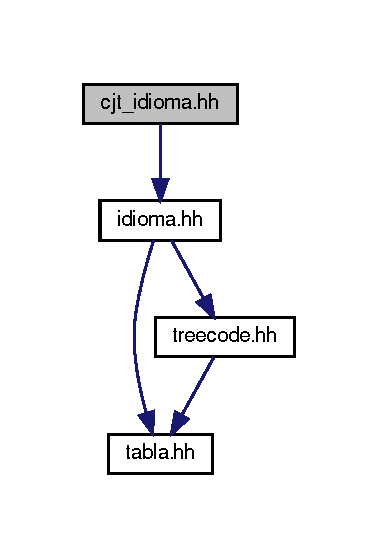
\includegraphics[width=182pt]{cjt__idioma_8hh__incl}
\end{center}
\end{figure}
\subsection*{Clases}
\begin{DoxyCompactItemize}
\item 
class \hyperlink{classcjt__idioma}{cjt\+\_\+idioma}
\begin{DoxyCompactList}\small\item\em Representa un conjunto de idomas. \end{DoxyCompactList}\end{DoxyCompactItemize}


\subsection{Descripción detallada}
Especificación de la clase cjt\+\_\+dioma. 


\hypertarget{idioma_8hh}{}\section{Referencia del Archivo idioma.\+hh}
\label{idioma_8hh}\index{idioma.\+hh@{idioma.\+hh}}


Especificación de la clase idioma.  


Dependencia gráfica adjunta para idioma.\+hh\+:\nopagebreak
\begin{figure}[H]
\begin{center}
\leavevmode
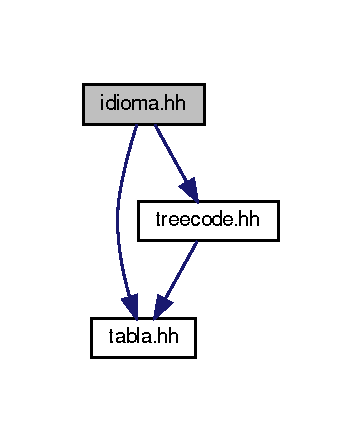
\includegraphics[width=174pt]{idioma_8hh__incl}
\end{center}
\end{figure}
\subsection*{Clases}
\begin{DoxyCompactItemize}
\item 
class \hyperlink{classidioma}{idioma}
\begin{DoxyCompactList}\small\item\em Representa un idoma. \end{DoxyCompactList}\end{DoxyCompactItemize}


\subsection{Descripción detallada}
Especificación de la clase idioma. 


\hypertarget{program_8cc}{}\section{Referencia del Archivo program.\+cc}
\label{program_8cc}\index{program.\+cc@{program.\+cc}}


Programa principal.  


Dependencia gráfica adjunta para program.\+cc\+:\nopagebreak
\begin{figure}[H]
\begin{center}
\leavevmode
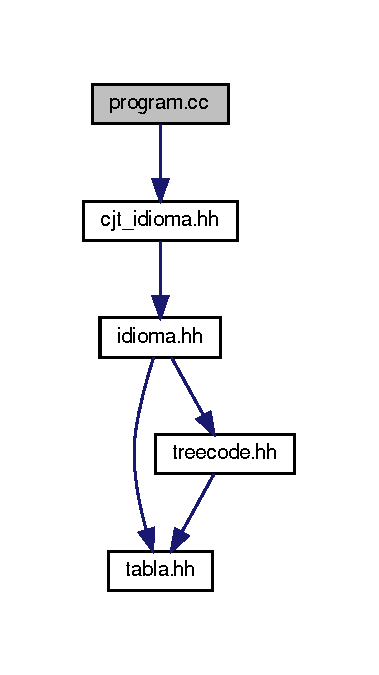
\includegraphics[width=182pt]{program_8cc__incl}
\end{center}
\end{figure}
\subsection*{Funciones}
\begin{DoxyCompactItemize}
\item 
int \hyperlink{program_8cc_ae66f6b31b5ad750f1fe042a706a4e3d4}{main} ()
\end{DoxyCompactItemize}


\subsection{Descripción detallada}
Programa principal. 



\subsection{Documentación de las funciones}
\mbox{\Hypertarget{program_8cc_ae66f6b31b5ad750f1fe042a706a4e3d4}\label{program_8cc_ae66f6b31b5ad750f1fe042a706a4e3d4}} 
\index{program.\+cc@{program.\+cc}!main@{main}}
\index{main@{main}!program.\+cc@{program.\+cc}}
\subsubsection{\texorpdfstring{main()}{main()}}
{\footnotesize\ttfamily int main (\begin{DoxyParamCaption}{ }\end{DoxyParamCaption})}



Definición en la línea 23 del archivo program.\+cc.


\begin{DoxyCode}
23           \{
24     \textcolor{keywordtype}{int} n;
25     cin >>n;
26     \hyperlink{classcjt__idioma}{cjt\_idioma} c;
27     \textcolor{keywordtype}{string} i;
28     \textcolor{keywordflow}{for}(\textcolor{keywordtype}{int} j=0; j<n; j++)\{
29         cin >> i;
30         c.\hyperlink{classcjt__idioma_aaf8acea2625eb1a72fbeaed23357c4ad}{anadir\_idioma}(i);
31     \}
32     \textcolor{keywordtype}{string} s;
33     \textcolor{keywordflow}{while}(cin>>s and s != \textcolor{stringliteral}{"fin"})\{
34         
35         \textcolor{keywordflow}{if}(s == \textcolor{stringliteral}{"anadir/modificar"})\{
36             cin >> i;
37             \textcolor{keywordflow}{if}(c.\hyperlink{classcjt__idioma_a253fbf0732efc679dea434ee7d261ffa}{existe\_idioma}(i)) c.\hyperlink{classcjt__idioma_ac9cdce411a32c42a9fc7da848f7de4c0}{modificar\_idioma}(i);
38             \textcolor{keywordflow}{else} \{
39                 c.\hyperlink{classcjt__idioma_aaf8acea2625eb1a72fbeaed23357c4ad}{anadir\_idioma}(i);
40                 cout << \textcolor{stringliteral}{"Anadido "} << i << endl<<endl;
41             \}
42         \}
43         
44         \textcolor{keywordflow}{else} \textcolor{keywordflow}{if}(s == \textcolor{stringliteral}{"codifica"})\{
45             cin >> i;
46             \textcolor{keywordtype}{string} texto;
47             cin >> texto;
48             cout<< \textcolor{stringliteral}{"Codifica en "} << i << \textcolor{stringliteral}{" el texto:"} << endl;
49             cout << texto << endl;
50             c.\hyperlink{classcjt__idioma_a5a92374dcbb5b9a0af7fdfccb59bc423}{codifica}(i, texto);
51         \}
52         
53         \textcolor{keywordflow}{else} \textcolor{keywordflow}{if}(s == \textcolor{stringliteral}{"decodifica"})\{
54             \textcolor{keywordtype}{string} texto;
55             cin >> i >> texto;
56             cout<< \textcolor{stringliteral}{"Decodifica en "} << i << \textcolor{stringliteral}{" el texto:"} << endl;
57             cout << texto << endl;
58             c.\hyperlink{classcjt__idioma_a25ee22b5af84a8ce22de2cee8128a08c}{decodifica}(i, texto);
59         \}
60         
61         
62         \textcolor{keywordflow}{else} \textcolor{keywordflow}{if}(s == \textcolor{stringliteral}{"tabla\_frec"})\{
63             cin >> i;
64             \textcolor{keywordflow}{if}(c.\hyperlink{classcjt__idioma_a253fbf0732efc679dea434ee7d261ffa}{existe\_idioma}(i))\{
65                 cout << \textcolor{stringliteral}{"Tabla de frecuencias de "} << i << \textcolor{stringliteral}{":"} << endl;
66                 c.\hyperlink{classcjt__idioma_ae2ab9ad48166bad14e113f748d1a888c}{consultar\_tabla\_de\_frequencias}(i);
67             \}
68             \textcolor{keywordflow}{else}\{
69                 cout << \textcolor{stringliteral}{"Tabla de frecuencias de "} << i << \textcolor{stringliteral}{":"} << endl;
70                 cout << \textcolor{stringliteral}{"El idioma no existe"}<< endl << endl;
71             \}
72         \}
73         
74         \textcolor{keywordflow}{else} \textcolor{keywordflow}{if}(s == \textcolor{stringliteral}{"treecode"})\{
75             cin >> i;
76             \textcolor{keywordflow}{if}(c.\hyperlink{classcjt__idioma_a253fbf0732efc679dea434ee7d261ffa}{existe\_idioma}(i))\{
77                 cout << \textcolor{stringliteral}{"Treecode de "} << i <<\textcolor{stringliteral}{":"}<< endl;
78                 c.\hyperlink{classcjt__idioma_a2d13a4e69a358756359ee6e262de2fb0}{consultar\_treecode}(i);
79             \}
80             \textcolor{keywordflow}{else}\{
81                 cout << \textcolor{stringliteral}{"Treecode de "} << i <<\textcolor{stringliteral}{":"}<< endl;
82                 cout << \textcolor{stringliteral}{"El idioma no existe"}<< endl << endl;
83             \}
84         \}
85     
86         \textcolor{keywordflow}{else} \textcolor{keywordflow}{if}(s == \textcolor{stringliteral}{"codigos"})\{
87                 cin >>i;
88                 c.\hyperlink{classcjt__idioma_a2e4b954ce7ee66596412c335430e9be8}{consultar\_codigos}(i);
89                 cout << endl;
90         \}      
91     \}
92 \}
\end{DoxyCode}

\hypertarget{tabla_8hh}{}\section{Referencia del Archivo tabla.\+hh}
\label{tabla_8hh}\index{tabla.\+hh@{tabla.\+hh}}


Especificación de la clase tabla.  


\subsection*{Clases}
\begin{DoxyCompactItemize}
\item 
class \hyperlink{classtabla}{tabla}
\begin{DoxyCompactList}\small\item\em Representa la tabla de frecuencias de un idioma. \end{DoxyCompactList}\end{DoxyCompactItemize}


\subsection{Descripción detallada}
Especificación de la clase tabla. 


\hypertarget{treecode_8hh}{}\section{Referencia del Archivo treecode.\+hh}
\label{treecode_8hh}\index{treecode.\+hh@{treecode.\+hh}}


Especificación de la clase treecode.  


Dependencia gráfica adjunta para treecode.\+hh\+:\nopagebreak
\begin{figure}[H]
\begin{center}
\leavevmode
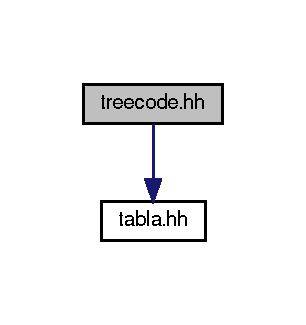
\includegraphics[width=147pt]{treecode_8hh__incl}
\end{center}
\end{figure}
\subsection*{Clases}
\begin{DoxyCompactItemize}
\item 
class \hyperlink{classtreecode}{treecode}
\begin{DoxyCompactList}\small\item\em Representa el treecode de un idioma. \end{DoxyCompactList}\end{DoxyCompactItemize}


\subsection{Descripción detallada}
Especificación de la clase treecode. 


%--- End generated contents ---

% Index
\backmatter
\newpage
\phantomsection
\clearemptydoublepage
\addcontentsline{toc}{chapter}{Índice}
\printindex

\end{document}
